%\section{Introduction}

%\cs{T}he Internet's routing infrastructure is made up of thousands of
%independently operated networks that cooperate to exchange global
%reachability information using an interdomain routing protocol, the
%Border Gateway Protocol, Version 4 (BGP)~\cite{rfc1771}.  

\cs{I}n~Internet routing, independently operated autonomous systems (ASes)
must cooperate to exchange global information; nevertheless, this
cooperation occurs in a landscape where these independent networks
compete to provide Internet service.  BGP
facilitates this ``competitive cooperation'' by enabling network
operators to express routing policies that are consistent with desired
economic, business, and performance goals.
%A key requirement of the competitive Internet landscape is that each
%AS be able to locally specify flexible policies, without
%revealing those policies to any other party.  

Recall from Section~\ref{sec:semantics} that {\em ranking} and {\em
filtering} are the two main mechanisms that operators use to implement
their policies.  Ranking determines which of many possible routes to a
destination should be used, thus providing an AS the flexibility to specify
preferences over multiple candidate paths to a destination (\eg,
specifying a primary and a backup path).  Filtering allows an AS to
selectively advertise routes to some ASes and hide routes
from others, thereby controlling which neighboring ASes
send traffic over its infrastructure.

There are two important characteristics of policy routing: {\em
autonomy} and {\em expressiveness}.  Autonomy is the ability of each
AS to set its rankings and filters independent of the others.
Expressiveness refers to the flexibility
that the routing protocol provides an operator for specifying rankings and
filters.  Ranking expressiveness determines what classes of rankings
over routes are permitted by the protocol, while filtering
expressiveness determines the range of route filters that are allowed.

The combination of expressiveness and autonomy has, in large part, been
the reason for the success of BGP over the past decade.  We contend that
both autonomy and filtering expressiveness will be {\em requirements}
for policy routing for the foreseeable future.  Previous studies of
routing stability assume that ASes are willing to compromise some degree
of autonomy, filtering expressiveness, or both (see
Section~\ref{sec:bg_stability}).  However, autonomy preserves each AS's
ability to set its policies without coordinating with any other AS.
Filtering expressiveness gives an AS flexibility in how it establishes
contracts with another AS, a task that should be unconstrained.
%For example, a very
%expressive protocol allows an AS to express any possible set of rankings
%over paths; a minimally expressive protocol would only allow ASes to
%prefer paths with shorter AS path lengths than longer ones.  

%Thus, the routing protocol
%should not impose any filtering restrictions.  We motivate the need for
%filtering expressiveness further in Section~\ref{sec:related}.

%% Expressive ranking and filtering form the cornerstone of interdomain
%% routing, 

Ideally, an interdomain routing system should preserve autonomy,
filtering expressiveness, and ranking expressiveness.  However, the
ability to specify highly expressive rankings comes at considerable cost
to system robustness: as has been observed by Varadhan \ea and Griffin
\eans, among others, if there are no constraints on the rankings that an
AS can specify, BGP may violate safety (\ie, oscillate
forever)~\cite{Griffin2002c,Varadhan1996}.

%Since providers must use both ranking and filtering to encode their
%policy decisions, it it imperative that they be able to do so with
%minimal restrictions and independently of other ASes.  

%Because a neighbor can send traffic through an AS only if the
%corresponding route were advertised to it, and carrying traffic incurs
%cost, filtering is an invaluable way to codify business relationships
%between ASes.

%% A key design requirement of policy-based routing is that each AS should
%% be able to specify their policies independently of how other ASes
%% specify their policies; that is, policy specification should be {\em
%% autonomous}.  Autonomous policy specification allows the routing system
%% to cooperate without requiring ASes to coordinate their policies or to
%% divulge potentially sensitive information (since rankings and route
%% advertisement implicitly encode business arrangements).

\begin{example}
\label{ex:intro1}
Consider Figure~\ref{fig:bg1}~\cite{Griffin2002c,Varadhan1996}.  ASes
$1$, $2$, and $3$ each prefer the indirect path through their
neighboring AS in the clockwise direction over the direct path to the
destination, $0$.  All other paths are filtered. This configuration has
no stable path assignment (\ie, a path assignment from which no node
would deviate).
% any path assignment that involves a direct path between an
%AS and the destination causes the AS in the counterclockwise direction
%to switch to using that path, thus forcing the AS in the clockwise
%direction to use the direct path.  
For example, consider the path assignment $(10, 210, 30)$; in this case,
AS $1$ has a better path available, $130$, so it switches paths.
This switch breaks the path $210$, causing AS $2$ to switch
to its second choice, path $20$.  The resulting path assignment,
$(130, 20, 30)$, is a permutation of the original path assignment: this
time, AS $3$ has the path $320$ available, so it switches.  This
oscillation continues forever.
\end{example}


\begin{figure}
\centerline{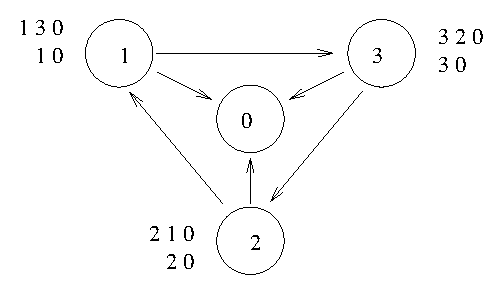
\epsfig{file=policy/figures/bg1.eps,width=0.5\textwidth}}
\caption[Safety violation caused by conflicting rankings in different
  ASes]{Instability can arise when each AS independently specifies 
  rankings~\protect\cite{Griffin2002c,Varadhan1996}. Each circle
  represents an AS.  AS $0$ is the destination.  The listing of paths
  beside each node denotes a ranking over paths.}
\label{fig:bg1}
\end{figure}

As the previous example suggests, full autonomy and expressiveness can
have undesirable consequences.  Routing protocol update messages
should reflect actual reachability changes in the network topology or
policy.  Unfortunately, in BGP, conflicting policies can cause
oscillations that produce endless streams of routing updates that are
unrelated to changes in topology or policy.  This instability creates
numerous performance problems, may cause network partitions, and
complicates diagnosis and debugging of problems in the routing
system.
%% but at least as
%% troubling is the fact that the protocol dynamics are difficult to reason
%% about: a network operator cannot determine if BGP routing updates are
%% caused by policy conflicts. 
Worse yet, a network operator has no way to guarantee that any given
configuration of rankings and filters will not adversely interact with
the policies of other ASes.  In light of these issues, developing
rigorous conditions on policy expressiveness that guarantee routing
stability, while preserving autonomy, is crucial.

This chapter explores the following question: provided that each AS
retains complete autonomy and complete filtering expressiveness, how
expressive can rankings be while guaranteeing stable routing?  This
question is important because ranking autonomy and filtering
expressiveness reflect the realities of how ASes specify policies today,
and little is known (beyond the results surveyed in
Section~\ref{sec:bg_stability}) about the tradeoffs between autonomy and
expressiveness as far as routing stability is concerned, particularly
under filtering.  In particular, our work is the first to develop
necessary conditions for stability under realistic assumptions about
autonomy and expressiveness and the first to derive necessary conditions
for stability in policy routing.


%Second, answering this question deepens understanding
%of stability of policy-based routing protocols, complementing earlier
%results by Varadhan \eans~\cite{Varadhan1996}, Griffin
%\eans~\cite{Griffin2002c}, and Gao and Rexford~\cite{Gao2001a}
%(Section~\ref{sec:related}).  

%% Our work is the first to present rigorous
%% theoretical results that suggest the constraints that should be placed
%% on routing policies to guarantee stability (regardless of network
%% operator decisions) while still preserving the autonomy of each AS.

%In light of this discovery, a natural question to ask is: ``What are
%the necessary and sufficient conditions that guarantee global routing
%stability?''  This question is rather broad, because these conditions
%depend on various modeling decisions: the details of the routing
%protocol, restrictions on
%filtering, and whether ASes retain policy independence.  
%This paper
%studies how the rankings allowed by a routing protocol must be restricted to
%guarantee global routing 
%stability, assuming that ASes (1)~retain ranking independence and
%(2)~face no restrictions on filtering.  

This chapter makes three main contributions.  First, in
Section~\ref{ssec:nhp}, we show that rankings based solely on the
immediate next-hop AS en route to the destination may never reach a
stable path assignment from an arbitrary initial state; \ie, next-hop
rankings, which are common in practice, are {\em not safe}.  Moreover,
under unrestricted filtering, a routing system with next-hop rankings
may have no stable path assignment.  In addition to their operational
implications, these results are also somewhat surprising, because
next-hop rankings with no route filtering always have one stable path
assignment.  We also observe that although rankings
based on a globally consistent weighting of paths are safe under
filtering, even minor generalizations of the weighting function
compromise safety (Section~\ref{ssec:ew}).

Second, we define a {\em dispute ring}, a special case of the
``dispute wheel'' (a group of nodes whose rankings have a particular
form) of Griffin
\ea\cite{Griffin2002c}, and show that any routing protocol that has
a dispute ring is not safe under filtering (Section~\ref{sec:dw}).
Using the dispute wheel concept, Griffin \ea showed a sufficient
condition for safety, proving that if a routing system is unsafe then
it must have a dispute wheel.  In contrast, to our knowledge, our
result is the first known necessary condition for safety under
filtering.

Third, we show that, providing for complete autonomy and filtering
expressiveness, the set of allowable rankings that guarantee safety is
effectively ranking based on variants of weighted shortest paths.  In
Section~\ref{sec:local}, we prove that any routing system that permits
paths of length $n+2$ to be ranked over paths of length $n$ can have a
dispute ring, and is thus unsafe under filtering.  We also prove that
any routing system that permits paths of length $n+1$ to be ranked over
paths of length $n$ can have a dispute wheel.  In summary, our results
indicate that stable policy routing with provider autonomy and
expressive filtering requires tight constraints on rankings.

Recent work has observed that routing protocols whose rankings are
derived from a ``strictly monotonic'' algebra are guaranteed to
converge~\cite{Griffin2005}; informally, a strictly monotonic algebra is
one where a path has a higher cost (\ie, is less preferred) than any
of its
subpaths.  In cases of unrestricted filtering,
these strictly monotonic algebras represent a generalization of shortest
paths routing, which is consistent with our results.  In
Section~\ref{sec:policy:implications}, we explain how both our results
and this algebraic framework lend insight into the design of future
policy-based routing protocols.


%, {\em for
%arbitrary and unrestricted filtering, guaranteeing that the routing
%will converge to a stable path assignment essentially requires to rank
%routes based on AS-path lengths}.


%Restricting only the rankings ensures complete autonomy for an AS:
%Unrestricted filtering permits ASes to engage in a wide
%variety of business relationships with other ASes.
%, unlike in Gao and
%Rexford's work where these relationships are constrained.  

%% We analyze the stability properties of various restrictions on route
%% rankings by defining and developing a {\em local
%% verifier} that each AS can use to determine whether the rankings it
%% has specified might violate stability.  
%% We show that the rules in our verifier are the ``tightest'' possible
%% constraints that can work with only local information, in the sense
%% that there is some network topology and filter specification in which
%% any relaxation of those rules will lead to instability.

Our findings may be interpreted in several ways.  The optimist will note
that checking a set of rankings to ensure safety is trivial, because all
it requires is that BGP routers modify the decision process to consult a
route's ``local preference'' attribute only after considering its AS
path length.  The pessimist, however, may conclude that guaranteeing
safe routing while preserving autonomy may yield constraints on
expressiveness that are too constraining.  In either case, the results
proved in this chapter about the fundamental tradeoff between the
expressiveness and autonomy may help guide the design of stable
interdomain routing protocols in the future;
Section~\ref{sec:policy:implications} explores some possibilities.

%% The rest of the paper is organized as follows.
%% Section~\ref{sec:related} provides background material and puts the
%% results in this paper in the context of relevant related work.
%% Section~\ref{sec:notation} formally presents our routing system model,
%% introducing notation and terminology.  Section~\ref{sec:nexthop}
%% examines the stability properties of two natural classes of
%% rankings---next-hop preferences and edge weight-based preferences---and
%% shows that the former is not guaranteed to be safe, while the latter
%% will always be safe, even under filtering.  Section~\ref{sec:dw} defines
%% two static constructs for analyzing stability---dispute wheel
%% (originally defined by Griffin \ea) and the dispute ring---and
%% presents new results on stability and safety.  Section~\ref{sec:local}
%% introduces {\em local verifiers} and derives constraints on local
%% rankings that must be satisfied to guarantee stability.
%% Section~\ref{sec:conclusion} discusses the implications of our results
%% and concludes.

%XXX need a concluding sentence
%here; it does not matter if it ends on a melancholy tone.



%% After discussing related work in
%% Section~\ref{sec:related}, we present our routing model in
%% Section~\ref{sec:notation} and 
%% formally define {\em safety}, 
%% a property stating that the routing system that converges, regardless of
%% the initial 
%% path assignment and ordering of routing messages.
%% In Section~\ref{sec:nexthop}, we study the stability properties of two
%% natural classes of  
%% rankings that preserve ranking independence: those based solely on the
%% immediate next-hop AS en route to 
%% the destination (``next-hop rankings'') and those based on a globally
%% consistent weighting of paths (``edge weight-based rankings'').  Although
%% next-hop rankings are commonly used in practice, we find, nevertheless,
%% that they may be unsafe.  We then 
%% note that rankings 
%% based on shortest path routing are safe, even under
%% filtering, but that 
%% a more general class of rankings based on edge weights is unsafe.

%% In light of these findings, it is natural to ask whether {\em any}
%% protocol other than shortest paths routing 
%% both preserves ranking independence and is safe
%% under unrestricted filtering.  To answer this question, in
%% Section~\ref{sec:dw}, we introduce the 
%% concept of a 
%% %We first show that under unrestricted filters, a routing system that has
%% a \emph{dispute ring} (a special case of the dispute
%% {\em wheel} concept introduced by Griffin \ea\cite{Griffin2002c})
%% and prove that under unrestricted filtering, a routing system that has a
%% dispute ring
%% is unsafe.
%% Using the dispute ring concept, we prove in
%% Section~\ref{sec:local} that {\em for arbitrary 
%% topologies and unrestricted filtering, guaranteeing that the routing
%% system will converge to a stable path assignment essentially requires
%% ASes to rank routes based on AS-path lengths}.
%% We then define a new abstraction that captures ranking independence,
%% called a {\em local
%%   verifier}, to 
%% prove that any routing system that permits paths of
%% length $n+2$ to be preferred over paths of length $n$ can have a dispute
%% ring, and is thus unsafe under unrestricted filtering.  We
%% also prove that any routing system that permits paths of length $n+1$ to
%% be preferred over paths of length $n$ can have a dispute wheel.
%% % (hence,
%% %these systems {\em may} have no stable routing).
